\documentclass[12pt,a4paper]{article}
\usepackage[printwatermark, disablegeometry]{xwatermark}
\usepackage{ACEEenrollment}
\usepackage{setspace}
\usepackage{fontspec}
\usepackage{indentfirst}
\usepackage{wallpaper}
\usepackage{mhchem}
\usepackage{hyperref}
\hypersetup{hidelinks}
\usepackage{etoolbox}%
\makeatletter
\patchcmd{\ttlh@hang}{\parindent\z@}{\parindent\z@\leavevmode}{}{}%
\patchcmd{\ttlh@hang}{\noindent}{}{}{}%
\makeatother

\renewcommand{\contentsname}{{\centerline{目录}}}
%\CenterWallPaper{0.8}{acee.png}
\setlength{\parindent}{2em}
\begin{document}
\begin{titlepage}
\ACEEtitle{2016}
\end{titlepage}
\begin{spacing}{2.2}
\tableofcontents
\end{spacing}
\ThisCenterWallPaper{0.8}{acee.png}
\newpage


\ThisCenterWallPaper{0.8}{acee.png}
\ACEEsection{工程筑梦}

\begin{spacing}{1.36}
{\kaishu \xiaosihao
\noindent 亲爱的同学:\par
我不熟悉你的音容笑貌,点点滴滴。我也不知道你来自何方,将向何去。但将与君言一语,请君为我倾耳听。\par
 与其说我们将成为同学,不如说我们将是这段旅程中相扶相持,携手并进的伴侣。隶属于竺可桢学院的工程教育高级班[Advanced Honor Class of Engineering Education]正是使我们相识相知,了解交流的平台。此时此刻,我们想问问你:工程是什么?工程师到底追求什么?这个科技爆炸的时代终能让我们向浩瀚星河发出更加强有力的呐喊,还是迎来永恒的静默?而你又打算在其中扮演怎样的角色?\par
是的,我们永远不能也不会给出你一个标准答案。因此,我们诚挚地邀请你加入我们思考的行列。你,一定和我们一样,绝不愿意把思维限于书本试卷中,而是置于声、光、电和广袤的天地。你,一定和我们一样,热爱手中的工具,愿意弄脏自己的手来创造点什么,乐哉其中。你,一定和我们一样,理智务实,深深明白实验和犯傻的区别,并愿意为了理想中的殿堂,竭尽全力搭好手头的一砖一宇。你,也一定和我们一样,永不满足,时时警醒,甚至疯狂到相信,世界一定会因你的前行而改变。\par
四年里,我将允诺你齐心协力的同伴,愿你应我以踽踽前行的坚毅。\par
十年中,我将赠与你照亮前路的火把,愿你返我以突破桎梏的勇气。\par
一辈子,我会赐予你披荆斩棘的剑器,愿你惠我以星河璀璨的天地。\par
欢迎踏入这场神秘的旅程!好戏才刚刚开始。\par
{\hspace*{0.7\textwidth}}{\fontspec{MATURASC.TTF}[Alternate=0]{\textbf{-}ACEERS}}}
\end{spacing}
\ThisCenterWallPaper{0.8}{acee.png}
%%%%%%%%%%%%%%%%%%%%%%%%%%%%%%%%%%%%%%%%%%%%%%%%%%%%%%%%%%
%%%%%%%%%%%填表说明%%%%%%%%%%%%%%%%%%%%%%%%%%%%%%%%%%%%%%%%%%
%%%%%%%%%%%%%%%%%%%%%%%%%%%%%%%%%%%%%%%%%%%%%%%%%%%%%%%%%%%%
\newpage
\phantomsection
\ACEEsection{填表说明}
\ThisCenterWallPaper{0.8}{acee.png}
\vspace*{5pt}
{\fang
\begin{enumerate}[label=\arabic*.]
\setlength{\itemsep}{0.5pt}
\item 此为资料册,其上内容仅供阅读,{\color{red}\bf{请勿在本表上直接作答,且本表不必打印上交}}。 
\item 填写报名表前,请{\color{red}\bf{务必于 3 月 25 日 16:00 前登陆浙江大学现代教务管理系统}},进入``专业确认'',点击``辅修报名'',在``申请专业''中选择``工高班''并进行报名确认。 
\item 请你将问题回答在``{\color{red}\bf{2016 浙江大学工程教育高级班报名表}}''的文件中,按原版式填写并转换成{\color{red} \bf{PDF 格式}}后打印,谢绝手写(保证及签名必须手写)。
\item 请将报名表的电子版({\color{red}\bf{PDF 格式}})、个人信息统计的 Excel 表格以及题目要求提交的文件打包压缩,在 {\color{red}\bf{3 月 25 日 13:00 之前}}将压缩文件发至邮箱:{\color{red}\bf{acee15\_enrollment@163.com}};邮件主题及压缩包文件均命名为``{\bf{学号+姓名+选做题题号}}'', 例如:``{\color{red}\bf{3150199422+龚皋+AC}}''。
\item 请在交表时间({\color{red}\bf{3 月 25 日 13:00-18:00}})将打印好的报名表连同纸质附件及其他必要材料交至紫金港校区{\color{red}\bf{小剧场B座306}}。\par 
纸质附件中必须包含: 
\begin{enumerate}[label=(\arabic*.)]
\setlength{\itemsep}{0pt}
\item 个人大学期间已修课程成绩单及最新的大类或专业综合排名,并加盖所在学院(园){\bf{成绩证明专用章}}。若无盖章视为无效(暂无排名同学请递交书面解释并且请所在学院(园)主管老师签字盖章)。
\item 至少一封浙大老师推荐信,辅导员除外。(提倡手写稿,也可为打印稿,但是要求有老师的手写签名或私人印章。)
\end{enumerate}
\item 在上交纸质材料时,若填表中提及所获奖项,请提交获奖证书复印件。允许附加任何你认为有必要的附件,请使用 A4 纸打印或复印。
\item 填表过程中请关注微信公众号``浙大工高班ACEE''以了解最新招生动态,交表后务必及时关注竺可桢学院办公网 http://ckc.zju.edu.cn 及 CC98 ACEE招生专楼以确定是否进入面试名单。
\item 对于有意向申请 ``{\color{red}\bf{中法 4+4}}''项目及``{\color{red}\bf{电气学院爱迪生班}}''的同学,不允许报名工高班。{\color{red}\bf{不接受已有辅修或计划报名其他特殊班级的同学}}。
\item 每份提交的报名表都未必完美,即便你没有按要求完成每一道题,这也不会决定最终的结果。希望你怀着一份执着,勇敢地展示已经取得的成果。
\item 在报名表中如有引用请注明参考资料来源。
\item 本资料册解释权归浙江大学竺可桢学院工程教育高级班所有。
\end{enumerate}
%%%%%%%%%%%%%%%%%%%%%%%%%%%%%%%%%%%%%%%%%%%%%%%%%%%%%%%
%%%%%%%%%%%%%%%%%%%Module 1%%%%%%%%%%%%%%%%%%%%%%%%%%%%
%%%%%%%%%%%%%%%%%%%%%%%%%%%%%%%%%%%%%%%%%%%%%%%%%%%%%%%
\newpage
\ThisCenterWallPaper{0.8}{acee.png}
}
%\end{spacing}
\phantomsection
\ACEEsection{ Module 1}
\begin{ACEEmodule}{1.4}{\xiaosihao}{\kaishu}
工高培育的工程师不是生硬枯燥的知识搬运家,不是头破血流的蛮横砖瓦匠,也绝不是不顾实际的异想天开者。人是所有社会关系的总和,我们每个人都需承当自己对这个社会的责任。工程师,应当是为改善人类生活而工作;工程精英,理应为全社会公共福祉而服务。众所周知,大家光辉如正午之日普照万物,科技魅力如皎皎明月辉惠世间。而在早已浑然一体的世界里,借助语言之梯,无论是大师还是顶尖技术,我们都能离他们更近一步。\par
这个模块里包含两个问题。请你将所获取的知识、信息和思考的硕果中最觉珍贵、最引以为豪的内容,以你认为最恰当、最有效的方式在报名表中表达出来,与我们分享。我们希望你知道:我们绝不会关注你的篇幅,但希望你能清晰地表达。同时,请不要在这两个问题的回答中添加附件。请按照学术规范写作,对涉及对他人观点、研究成果的引用,请务必以参考资料或参考文献的形式标明。\par
\end{ACEEmodule}

%%%%%%%%%%%%%%%%%%%%%%%%%%%%%%%%%%%%%%%%%%%%%%%%%%%%%%%%
%%%%%%%%%%%%%%%%%%%%%%%%%%%%%%%%%%%%%%%%%%%%%%%%%%%%%%%	Q1Q1Q1
%%%%%%%%%%%%%%%%%%%%%%%%%%%%%%%%%%%%%%%%%%%%%%%%%%%%%%%
\newpage
\ThisCenterWallPaper{0.8}{acee.png}
\phantomsection
\ACEEsubsection{Question 1}
\begin{ACEEquestion}{1.4}{\xiaosihao}{\youyuan}
我们知道,漠不关心社会问题的人,就像遇到海难逃到救生艇上的某些人一样。艇的一端有个洞,他们坐在艇的另一端,看着那端的人竭力舀水以免沉没。其中一个人说:``谢天谢地,那个洞不在我们这边。''的确,人是社会的动物。我们不可避免地会被时代影响,也会影响这个时代。从引力波到AlphaGo,工程急速地改变着人们的生活和未来。作为工程精英摇篮的工高旨在培养有经天纬地之才,担当宇宙的栋梁。现在,我们想请你畅想,你认为社会存在哪些可以通过技术革新改善的问题?而你愿意在这些方面做出怎样的改良?请结合具体事例阐明你的观点,注意逻辑性与简洁性。
\end{ACEEquestion}
%%%%%%%%%%%%%%%%%%%%%%%%%%%%%%%%%%%%%%%%%%%%%%%%%%%%%%%%%%%%%%%%%
%%%%%%%%%%%%%%%%%%%%%%%%%%%%%%%%%%%%%%%%%%%%%%%%%%%%%%%Q2Q2Q2Q2
%%%%%%%%%%%%%%%%%%%%%%%%%%%%%%%%%%%%%%%%%%%%%%%%%%%%%%%%%%%%%%%%%%%
\newpage
\ThisCenterWallPaper{0.8}{acee.png}
\ACEEsubsection{Question 2}
\begin{ACEEquestion}{1.2}{\xiaosihao}{\youyuan}
A foreign language is a power, like the wings of a bird and the windows of a house. \par 
语言是工具、武器,人们利用它来互相交际,交流思想,达到互相了解。身为理工类学生的你或许没有含蓄而优美的表达,但我们希望你能好好利用语言,去跟上世界科技的发展,触及伟人思想。\par
从下面三篇文献中任选一篇,请仔细阅读后完成对应的问题。文献均在``Question 2附件''文件夹中。\par

\begin{enumerate}[label=(\arabic*)]
\item Franc-Hlavac-DAGM05-B\par
数学是编程的灵魂,计算机和数学息息相关。该文献描述了计算机中马尔科夫链识别车牌的应用,请仔细阅读后谈谈你的启发,并有创意地设想和详细分析马尔科夫链的其他应用。\par
\item Water Jet Cutting\par
在过去的一年里,中国制造业遭遇寒潮,许多企业相继倒闭,大多数人对中国制造业失去信心。事实上,传统工业仍处于兴起、兴盛时期,尚待大力发展。通过引入、采用新技术,对其进行改造,提高生命力,是传统工业继续发展、适应工业现代化要求的重要转型途径。请仔细阅读该文献,并运用物理知识分析此加工工艺的发展过程,并对此工艺的未来改进提出自己的设想。\par
\item 摩尔定律\par
摩尔定律是英特尔创始人之一戈登·摩尔提出的,该定律已持续超过半世纪。该文献讲述了摩尔定律的未来,请仔细阅读后谈谈摩尔定律继续持续下去的可能性。如果认为能持续下去,请谈谈所需的技术。如果认为不行,请说明理由。\par
\end{enumerate}
\end{ACEEquestion}
\newpage		
\ThisCenterWallPaper{0.8}{acee.png}
%%%%%%%%%%%%%%%%%%%%%%Module2

\ACEEsection{Module 2}
\begin{ACEEmodule}{1.34}{\xiaosihao}{\kaishu}

整合信息与快速学习,是长远前行所需的重要能力。面对浩如烟海的信息,学会获取自己最需要的,将获取的信息以最快的方式进行学习吸收,整合优化,并为己所用正是在前行路上披荆斩棘的宝剑。同时,我们希望你知道,我们不仅仅希望你为解决问题而努力,我们更希望你能总结反思,汲取经验,为下一次的征程做好准备。

最远的路属于最坚定的灵魂。未来的征程荆棘丛生,幸运的是,有些旅程,当你迈出第一步时,最艰难的时刻已经过去。只要你矢志不移,奋勇向前,脚下的路会渐进平坦,眼前的风景会柳暗花明。
    
这个模块中包含两个部分。请你在两个部分中{\bf{\color{red} 各选取一个问题}}尝试解决。(如果同时做了AB题,按A题计分;如果同时做了CDEFG中任意两道或更多,按照前面一题计分)或许你从未接触过这些工具,对这些问题也不了解。但是校园内有资源丰富的平台,我们相信,通过你的努力和创造,一定能顺利地解决这些问题。或许你已经在这些领域有所建树,那么,我们希望你能带来独树一格,多种多样的解决方法。我们还希望你能记录解决的完整过程和感悟,并书写在报名表提供的空间里。你遇到的困难,解决方法,整个过程中思路的变化,心得体会或者其他相关内容都请记录在报名表中。

希望你享受解决这些问题的乐趣!

\end{ACEEmodule}		
\newpage

%%%%%%%%%%%%%%%%%%%%%%AAAAAAAAAAAAAAAAAAAAAAAAAAAAAAAAAAAAAAAAAAAAAAAA
\ACEEsubsection{Section 1}
%\ThisCenterWallPaper{0.8}{acee.png}
\ThisURCornerWallPaper{0.5}{acee.png}
%\addcontentsline{toc}{subsection}{Section 1}

\begin{spacing}{1.4}
{\kaishu {\xiaosihao
Matlab是理工科常用的一款软件,它提供了强大的处理功能。复杂的数学问题,一般都可以用它极其丰富的函数库而轻易解决。Matlab内容庞杂,但是初学者入手,仍可以比较容易地掌握其基本语句。其数据的基本操作单位就是数组(包括向量)。利用Matlab可以很方便地绘制各种曲线和方程图象。它的某些基本结构与C语言类似又自有其特色,例如循环结构的for循环就既继承了C的基本结构,又有所创新。
}}
\end{spacing}
\ACEEsubsubsection{Problem A: Interpolation}
\begin{ACEEproblem}{1.4}{\xiaosihao}{\youyuan}
\begin{spacing}{1.4}
在MATLAB中,有一些有趣且实用的插值函数,例如pchip、spline、interp、polyinterp等等。请对各插值函数进行比较并使用你认为最合适的插值函数画出左图中的图像(函数不限于上述几种)右图仅为参考。开始的代码已经给出:\par
开始的代码已经给出:\par
figure(`position', get( 0,`screensize'))\par
axes(`position', [ 0.1 0.1 0.8 0.8 ])\par
\end{spacing}

\begin{itemize}
	\item 温馨提示
	\begin{itemize}
		\item 使用ginput函数采集点。
	\end{itemize}
\end{itemize}

\begin{figure}[H]
\small
\centering

\includegraphics[width=8.5cm]{A.png}
\caption{Problem A} 
\end{figure} 
\end{ACEEproblem}

\begin{ACEEsubmit}{A}
\begin{itemize}
	\item 任务报告
	\begin{itemize}
		\item[] 其中必须包括以下内容:
		\item[1.] 体现出具体的解题思路。
		\item[2.] 完成该任务的过程中,你是如何解决遇到的问题的,以及你的心得体会。除此之外,如果你还有其他希望说明的,也可以一同在任务报告中体现。
	\end{itemize}
	\item 源代码
	\begin{itemize}
		\item 命名规则``Code\_姓名全拼小写\_学号''。
		\item 提交.m格式文件。
		\item 程序中30\%以上的语句需有注释。
	\end{itemize}
	\item 画好的图片
	\begin{itemize}
		\item 命名规则``Figure\_姓名\_学号''。
		\item 提交一个.jpg格式文件。
	\end{itemize}
\end{itemize}
\end{ACEEsubmit}
\ThisCenterWallPaper{0.8}{acee.png}
\newpage
%\ThisCenterWallPaper{0.8}{acee.png}
\ThisURCornerWallPaper{0.5}{acee.png}
%%%%%%%%%%%%BBBBBBBBBBBBBBBBBBBBBBBBBBBBBBBBBBBBBBBBBBBBBBBBBBBBBBBBBBBBB

\ACEEsubsubsection{Problem B: Logistic Regression}
\begin{ACEEproblem}{1.4}{\xiaosihao}{\youyuan}
\begin{spacing}{1.4}
逻辑回归(Logistic Regression)是一种广义的线性回归分析模型,常用于数据挖掘,疾病自动诊断,经济预测等领域。B题附件中的Data.xlsx表格是某公司历年招聘员工的记录。Test A和Test B栏分别列出了每位应聘者的得分。Flag表示该应聘者是否被录取,其中flag为1表示被录用,flag为0表示未被录用。\par
(1)以Test A得分为横坐标,以Test B得分为纵坐标,使用Matlab将Excel文件中的数据样本绘制在图中,如下图所示。请自选与示例不同的图例。\par
\begin{figure}[H]
\small
\centering
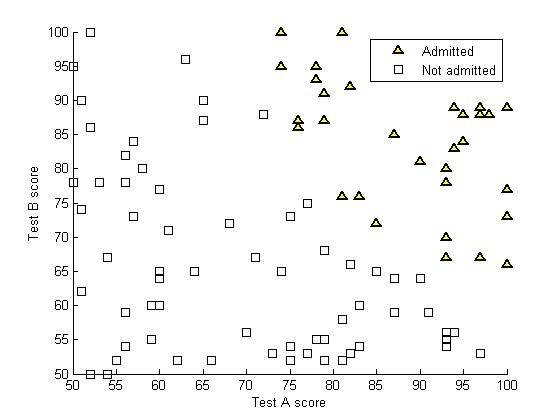
\includegraphics[width=12cm]{fig3.jpg}
\caption{Test A scores} \label{fig: area}
\end{figure} 
(2)通过已知样本,我们可以通过逻辑回归,对一个应聘者是否被录用做出预测。如图所示,请你在(1)中的样本分布图中作出如下图所示的两组样本的判别边界。	\par
\begin{figure}[H]
\small
\centering
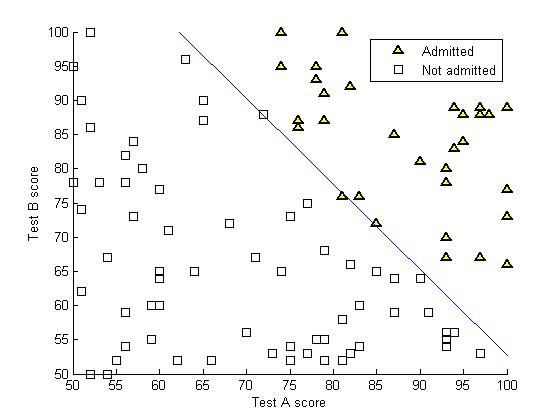
\includegraphics[width=12cm]{fig33.jpg}
\caption{Test A scores} 
\end{figure} 
\end{spacing}
\ThisLRCornerWallPaper{0.5}{acee.png}
\begin{itemize}
	\item 温馨提示
	\begin{itemize}
		\item[1.] 在Matlab中,fminunc函数可以高效的进行无约束优化。
		\item[2.] 计算成本函数与梯度的相应函数costFunction已在B题附件中给出,你可以在求解过程中利用该函数,并在M文件中添加充分的注释。
		\item[3.] 最基本的线性判别边界可以写成$\theta
		_0+\theta_1 x_1+\theta_2 x_2=0$的形式,其中$x_1 $和$x_2 $分别代表两个测试的分数。通常为了形式上的统一,令$x_0=1$, 写成$\theta_0 x_0+\theta_1 x_1+\theta_2 x_2=0$的形式。因此,你需要对原始数据矩阵做相应调整。
	\end{itemize}
\end{itemize}
\end{ACEEproblem}
%\begin{enumerate}[$\blacksquare$]{1.4}
%\ThisCenterWallPaper{0.8}{acee.png}
\begin{ACEEsubmit}{B}
\begin{itemize}
	\item 任务报告
		\begin{itemize}
			\item[] 其中必须包括以下内容:
			\item[1.] 含判别边界的应聘者数据散点图。
			\item[2.] 具体的解题思路。
			\item[3.] 完成该任务的过程中,你是如何解决遇到的问题的,以及你的心得体会。除此之外,如果你还有其他希望说明的,也可以一同在任务报告中体现。
		\end{itemize}
	\item 源代码
		\begin{itemize}
			\item[1.] 命名规则:``Code\_姓名全拼小写\_学号''。
			\item[2.] 添加了注释后的costFunction:``costFunction\_姓名全拼小写\_学号''。
			\item[3.] 提交.m格式文件。
			\item[4.] 程序中有足够的注释以体现对该问题的理解。 
		\end{itemize}
\end{itemize}
\end{ACEEsubmit}
\ThisCenterWallPaper{0.8}{acee.png}
\clearpage
\ACEEsubsection{Section 2}
%\ThisCenterWallPaper{0.8}{acee.png}
\ThisLRCornerWallPaper{0.5}{acee.png}
%\addcontentsline{toc}{section}{Section 2}
%%%%%%%%%%%5CCCCCCCCCCCCCCCCCCCCCCCCCCCCCCCCCCCCCCCCCCCC
\ACEEsubsubsection{Problem C: SolidWorks}
\begin{ACEEproblem}{1.05}{\xiaosihao}{\youyuan}
Solidworks 是一款非常实用的三维建模软件,并且 Solidworks 软件也非常容易上手。它良好的界面设计,强大的帮助功能可以让未接触过该软件的使用者迅速掌握基本的操作,进行三维设计。\par
下图是一个手摇风扇,它由 6 个构件组成:\par
\begin{figure}[H]
\small
\centering
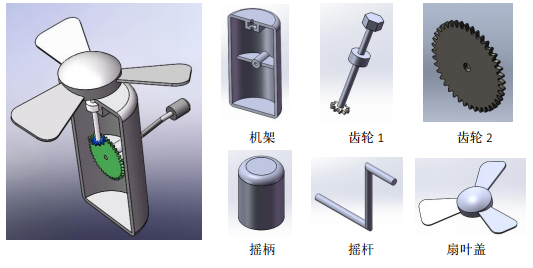
\includegraphics[width=10cm]{fig4.png}
\caption{手摇风扇} 
\end{figure} 
其中 机架、齿轮2、摇杆、扇叶盖未完成。请根据附件中的工程图,分别利用 SolidWorks 设计出对应的零件模型,并组成装配体。\par
\begin{itemize}
	\item 题目要求
	\begin{itemize}
		\item[1.] 所提交材料中应包括完成后的零件和装配体文件。要求几何关系明确,尺寸明确,草图完全定义。
		\item[2.] 零件材质不作要求。
		\item[3.] 如果需要使用SolidWorks的设计库,请选择中国标准(GB)。
	\end{itemize}
	\item 温馨提示
	\begin{itemize}
		\item[1.] 学习SolidWorks软件,遇到问题可以使用软件内置的帮助功能。
		\item[2.] 请使用2014或2015版本(紫金港机房有此软件)。
		\item[3.] 尝试使用 拉伸、旋转、扫描、拉伸切除、旋转切除、圆角、圆周阵列以及设计库中的Toolbox来帮助完成零件的设计。
	\end{itemize}
	\item 附件
	\begin{itemize}
		\item[] 见``C题附件''文件夹
	\end{itemize}
\end{itemize}
\ThisURCornerWallPaper{0.5}{acee.png}
\end{ACEEproblem}
\begin{ACEEsubmit}{C}
\begin{itemize}
	\item 任务报告
	\begin{itemize}
		\item[] 其中必须包括以下内容:
		\item[1.] 体现出具体的解题思路。
		\item[2.] 完成该任务的过程中,你是如何解决遇到的问题的,以及你的心得体会。除此之外,如果你还有其他希望说明的,也可以一同在任务报告中体现。
	\end{itemize}
	\item 源代码
	\begin{itemize}
		\item[] 所提交的各个文件分别以 ``齿轮1''、``齿轮2''、``机架''、``扇叶盖''、``摇柄''、``摇杆''、 ``手摇风扇(装配体)''命名。
		\begin{figure}[H]
			\small
			\centering
			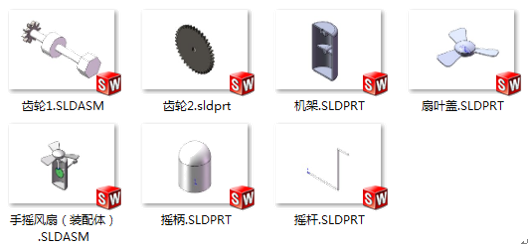
\includegraphics[width=10cm]{fig5.png}
			\caption{SolidWorks需提交的零件} 
		\end{figure} 
	\end{itemize}
\end{itemize}

%\ThisCenterWallPaper{0.8}{acee.png}
\end{ACEEsubmit}
\newpage
%\ThisCenterWallPaper{0.8}{acee.png}
%\ThisURCornerWallPaper{0.5}{acee.png}
%\ThisCenterWallPaper{0.8}{acee.png}
%%%%%%%%%%%%%%%%%%%5DDDDDDDDDDDDDDDDDDDDDDDDDDDDDDDDDDDDDDDDDDDDDDDDDDDDDDD

\ACEEsubsubsection{Problem D: Multisim}
\begin{ACEEproblem}{1.4}{\xiaosihao}{\youyuan}
Multisim是一款广泛应用的仿真工具,适用于板级的模拟/数字电路板的设计工作。现在,我们希望你学习运用这款软件,结合一定的数字电路知识,完成下面的任务:\par
(1)一名工高学长因创造了一项尖端发明而被间谍控制。为了更好地建设社会主义,现在请你破解密码,解救学长。你发现每个数字的二进制码采用以三为key的凯撒密码加密。比如,数字0对应的密码为0011,数字9对应的密码为1100。请你只用门电路,设计一个密码转换电路,实现破解。你需用Multisim画出转化电路图,其输入为待破解密码,输出为转换结果,结果用PROBE表示。请将你的学号的最后一位按照密码规则转换,作为测试样例输入,并将结果截图,与电路图一起附在提交文件中。\par
%\begin{figure}[H]
%\small
%\centering
%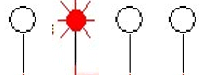
\includegraphics[width=12cm]{fig6.png}
%\caption{Problem D} \label{fig: area}
%\end{figure} 

(2)现在你已经成功破解密码,接近学长。为了证明身份,你被要求说明所属组织。请设计一个电路,用数码管显示ACEE和一个5-4-3-2-1-0的倒计时数字序列。需要注意的是,这一问的输入没有要求。在设计过程中,你可以运用门电路,也可以应用组装好的芯片。\par
你可能用到的有:74LS74,四个SEVEN\_SEG\_COM\_K数码管,一个DCD\_HEX数码管,CLOCK\_VOLTAGE,门电路和电阻。\par

%\begin{figure}[H]
%\small
%\centering
%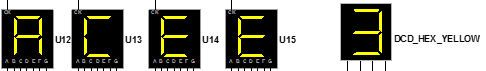
\includegraphics[width=12cm]{fig7.png}
%\caption{Problem D} \label{fig: area}
%\end{figure} 
%\end{spacing}


\ThisCenterWallPaper{0.8}{acee.png}
\begin{itemize}
	\item 温馨提示
	\begin{itemize}
		\item[1.] 不同的数字可以用不同的码制表示。卡诺图可以化简逻辑表达式。
		\item[2.] 数字电路中,不用的管脚应尽量不悬空,并根据其功用接入高低电平,防止信号干扰。
		\item[3.] 74LS74是一个双D触发器,功能图在附件中。
		\item[4.] 为了防止数码管被烧坏,通常需要在合适的位置加上保护电阻。
	\end{itemize}
\end{itemize}
\end{ACEEproblem}
\ThisCenterWallPaper{0.8}{acee.png}
\begin{ACEEsubmit}{D}
\begin{itemize}
	\item 任务报告
	\begin{itemize}
		\item[] 其中必须包括以下内容:
		\item[1.] 简述你的设计思路和得到逻辑表达式的过程。
		\item[2.] 完成该任务的过程中,你是如何解决遇到的问题的,及你的心得体会。除此之外,如果你还有其他希望说明的,也可以一同在任务报告中体现。
	\end{itemize}
	\item 源文件
	\begin{itemize}
		\item[1.] 命名规则``Multisim\_姓名\_学号''。
		\item[2.] 提交.ms格式文件。
	\end{itemize}	
\end{itemize}
\end{ACEEsubmit}
	\ThisCenterWallPaper{0.8}{acee.png}
%%%%%%%%%%%%%%%%%%%%%%%%EEEEEEEEEEEEEE
\newpage
\ThisCenterWallPaper{0.8}{acee.png}


\ACEEsubsubsection{Problem E: R} 
\begin{ACEEproblem}{1.4}{\xiaosihao}{\youyuan}
R 是一个自由软件,主要用于统计计算和统计制图。在生物统计方面,R已经被广泛使用。现在请你利用R完成一项关于生物统计的简单工作。你将得到两个数据集``2712qc.bim''和``E001-H3K4me1.narrowPeak'',两张数据集的基本信息见附件。\par
在数据集``2712qc.bim''中,每一行代表一条基因信息,每一条基因信息有五列数据:第一列表示所在染色体的名称,``1''即为1号染色体;第二列为资源标识符(rsid),每一条基因信息的资源标识符均不同;第三列表示基因在染色体上的位置(pos);第四、第五列表示基因中碱基对的种类。\par
在数据集``E001-H3K4me1.narrowPeak''中,每一行代表一条基因信息,每一条基因信息有十列数据,其中与本题相关的只有前三列数据:第一列表示所在染色体的名称,``chr1''即为1号染色体;第二列和第三列表示该基因在染色体上的位点(pos),所以第二第三列形成一个位点区间,后面均为基因位点的其他信息。\par
现在,你的任务是:对1到22号染色体中数据集已有的所有基因信息,找出每个位点所在的位点区间。即在数据集``2712qc.bim''中,根据所在染色体和所在染色体上的位点(pos),在数据集``E001-H3K4me1.narrowPeak''中找到其位点所在区间,并生成一个新的数据集。预期生成的数据集见附件。\par
\vspace*{4pt}
\begin{itemize}
	\item 温馨提示
	\begin{itemize}
		\item[1.] 对于没有找到对应信息的基因数据直接删掉即可。
		\item[2.] 只考虑1-22号染色体。
		\item[3.] 在解决此问题的过程中,可能会用到sapply函数。
		\item[4.] R中的包很多,但在本问题中你并不一定需要加载其他的包。
	\end{itemize}
\end{itemize}
\end{ACEEproblem}
\ThisCenterWallPaper{0.8}{acee.png}
\begin{ACEEsubmit}{E}
\begin{itemize}
	\item 任务报告
	\begin{itemize}
		\item[] 其中必须包括以下内容:
		\item[1.] 体现出具体的解题思路。
		\item[2.] 完成该任务的过程中,你是如何解决遇到的问题的,以及你的心得体会。除此之外,如果你还有其他希望说明的,也可以一同在任务报告中体现。
	\end{itemize}
	\item 源文件
	\begin{itemize}
		\item[1.] 代码文件命名为``R\_姓名全拼小写\_学号.R''。
		\item[2.] 生成的数据集命名为``R\_姓名全拼小写\_学号.csv''。
	\end{itemize}
\end{itemize}
\end{ACEEsubmit}
\newpage
%\ThisCenterWallPaper{0.8}{acee.png}
\ThisLRCornerWallPaper{0.5}{acee.png}
%%%%%%%%%%%%%%FFFFFFFFFFFFFFFFFFFFFFFFFFFFFFFFFFFFFFF
\phantomsection
\ACEEsubsubsection{Problem F: Python}
\begin{ACEEproblem}{1.4}{\xiaosihao}{\youyuan}
Python是一门十分强大的语言,利用Python可以实现许多好玩的功能,比如你想实时抓取一些网站的最新信息,就可以利用Python来实现。下面提供几个例子:\par
{\bf{案例一:}}\par
小明十分喜欢逛知乎,但是他发现总有很多这样的用户:他们拥有很多粉丝,但是几乎没什么有价值的答案,也就是存在``刷粉''现象。于是小明决定查查某个人的粉丝属于什么群体,来判断其是否可能``刷粉'',他利用Python读取了某个知乎用户所有粉丝的四个信息(关注者、提问、回答、赞同),然后统计四个数据都是零的粉丝(如下图)数目,这样可以初步判断是不是``僵尸粉''。\par
\begin{figure}[H]
\small
\centering

\includegraphics[width=12cm]{fig11.png}
\caption{Problem F}
\end{figure} 
{\bf{案例二:}}\par
小刚喜欢看百度贴吧里的美女图片,于是他想把``模特吧''里的某个帖子里的图片都下载下来,但是一张一张点太慢,他就利用Python把某个帖子里的图片全都存到指定目录下,慢慢欣赏。\par
\vspace*{4pt}
现在,请你利用Python来抓取自己感兴趣的信息,网站不限,内容不限(但不要违反相关法律法规),在提交的代码中要求有不少于30\%的注释,并且在代码最上方利用注释写出这个代码的作用。\par
\vspace*{4pt}

\begin{itemize}
	\item 温馨提示
	\begin{itemize}
		\item[1.] 我们会进行严格的代码查重,所以不要随意复制别人的代码来使用
		\item[2.] 请在提交时注明你运行代码所使用的Python版本
		\item[3.] Python有很多很好用的库,可自行学习,如要用到一些标准库以外的第三方库,请在附件文档中说明。
		\item[4.] 就算程序比较简单也没有关系,关键是学习的过程
	\end{itemize}
\end{itemize}
\end{ACEEproblem}
\ThisCenterWallPaper{0.8}{acee.png}
\begin{ACEEsubmit}{F}
\begin{itemize}
	\item 任务报告
		\begin{itemize}
			\item[] 其中必须包括以下内容:
			\item[1.] 体现出具体的解题思路。
			\item[2.] 完成该任务的过程中,你是如何解决遇到的问题的,以及你的心得体会。除此之外,如果你还有其他希望说明的,也可以一同在任务报告中体现。
		\end{itemize}
	\item 源代码
		\begin{itemize}
			\item[1.] 命名规则``Code\_姓名\_学号''。 
			\item[2.] 提交.py格式文件
		\end{itemize}
\end{itemize}
\end{ACEEsubmit}
%%%%%%%%%%GGGGGGGGGGGGGGGGGGGGGGGGGG
\newpage
\ThisCenterWallPaper{0.8}{acee.png}
\ACEEsubsubsection{Problem G: CrystalMaker}
\begin{ACEEproblem}{1.4}{\xiaosihao}{\youyuan}
晶体是常见的物质形态,其最基本的特点是具有长程有序的周期结构。想必你对晶体的宏观性质已经有一定的了解:如具有特定的熔沸点、硬度、不同的晶粒形貌,等等。事实上绝大部分的宏观属性是由其微观结构决定的,而当我们将目光放到晶体的微观结构上对晶体进行研究,第一步就是要构建晶体的围观模型:想象如何通过一个个的原子来搭建基元,然后按照一定的规则作周期延拓而得到晶体。在这一方面,CrystalMaker是一个十分常用且方便操作的可视化软件。\par
请你在理解好``基元''、``晶格''、``晶格常数''等基本概念的基础上,查阅相关资料,利用CrystalMaker软件,绘制以下三种晶体的三维模型:\par

\begin{center}
{\ce{GaAs}} \hspace{0.2\textwidth}     {\ce{SiO2}} \hspace{0.2\textwidth}     {\ce{diamond}}
\end{center}
%\vspace*{-\baselineskip}
\vspace*{4pt}
%\\[0.2\baselineskip]
\begin{itemize}
	\item 温馨提示
	\begin{itemize}
		\item[] 应当充分考虑各个晶体的相关参数,尽可能精确地反应晶体的空间结构特性
	\end{itemize}
\end{itemize}
\end{ACEEproblem}
\clearpage
\ThisCenterWallPaper{0.8}{acee.png}
\begin{ACEEsubmit}{G}
	\begin{itemize}
		\item 任务报告
		\begin{itemize}
			\item[] 其中必须包括以下内容:
			\item[1.] 体现出具体的解题思路。
			\item[2.] 请说明这三种晶体分别属于什么晶格类型、说明(可以辅以图解)基元的组成,说明三者的异同。
			\item[3.] 仅要求显示一个合适的晶胞,可以形象地反应晶体的周期性结构即可,在此基础上,每个晶体选择合适的视角截取三个视图附到你的报告中,要求能尽可能形象地表现晶体的立体结构。
			\item[4.] 完成该任务的过程中,你是如何解决遇到的问题的,以及你的心得体会。除此之外,如果你还有其他希望说明的,也可以一同在任务报告中体现。
		\end{itemize}	
		\item 源文件
		\begin{itemize}
			\item[] 请提交.cdmf文件,命名格式为``学号\_晶体名.cdmf''。
		\end{itemize}
	\end{itemize}
\end{ACEEsubmit}

\end{document}